\documentclass{article}

\usepackage{amsmath}
\usepackage{amssymb}
\usepackage{graphicx}
\usepackage[spanish]{babel}
\usepackage{cancel}
\usepackage{enumerate}
\usepackage{hyperref}
\hypersetup{
    colorlinks,
    citecolor=black,
    filecolor=black,
    linkcolor=black,
    urlcolor=black,
}
\usepackage{tcolorbox}
\usepackage{xcolor}

\tcbuselibrary{theorems}

\newcommand{\hresult}[2]{\tcboxmath[colback=orange!25!white,colframe=orange, title=#1] {#2} }
\newcommand{\hresulte}[3]{\tcboxmath[colback=orange!25!white,colframe=orange, title=#1] { \hspace{#3} #2 \hspace{#3} } }

\renewcommand{\Bbb}{\mathbb}

\title{Ejercicios de Análisis Matemático CBC (28) \\
Práctica 1: Funciones reales \\
Cátedra Ruiz, curso 62802 \\
1° C 2003}
\author{Darío Eduardo Ramos}

\begin{document}
\maketitle

\tableofcontents{}

\newpage

\section*{1}
\label{sec:1}
\addcontentsline{toc}{section}{\nameref{sec:1}}

\textbf{Haga un gráfico que refleje la evolución de la temperatura del agua a lo largo del tiempo atendiendo a la siguiente descripción:}

\vspace{1em}

\textbf{``Saqué del fuego una cacerola con agua hirviendo. Al principio, la temperatura del agua bajó con rapidez, de modo que a los 5 minutos estaba en 60º. Luego fue enfriándose con más lentitud. A los 20 minutos de haberla sacado estaba a 30º y 20 minutos después seguía teniendo algo más de 20º, temperatura de la cual no bajó, pues era la temperatura que había en la cocina.'' }

\vspace{1em}

\textbf{¿Es el gráfico que hizo el único que respeta las consignas anteriores?}

\vspace{1em}

\hrule

\vspace{1em}

Planteando la temperatura como una función del tiempo, llámese $y = f(t)$, los datos que se tienen sobre $f$ son los siguientes:

\begin{subequations}
\begin{align}
& f(t < 0) = 100 \\
& f(0) = 100 \\
& f(5) = 60 \\
& f(20) = 30 \\
& f(40) = 20+ \\
& f(t > 40) = 20
\end{align}
\end{subequations}

Dado que no se tiene una expresión cerrada para $f$, existen infinitas funciones de variable continua que satisfacen estas restricciones. Cualquier gráfico que se haga que pase por los puntos dados y se mantenga constante para $t < 0$ y $t > 40$ con los valores dados es válido. Resulta conveniente definir los grados Celsius como la unidad del eje $y$, y los minutos como la unidad del eje $x$. Por ejemplo:

\newpage

\begin{figure}[ht]
\caption{un gráfico posible}
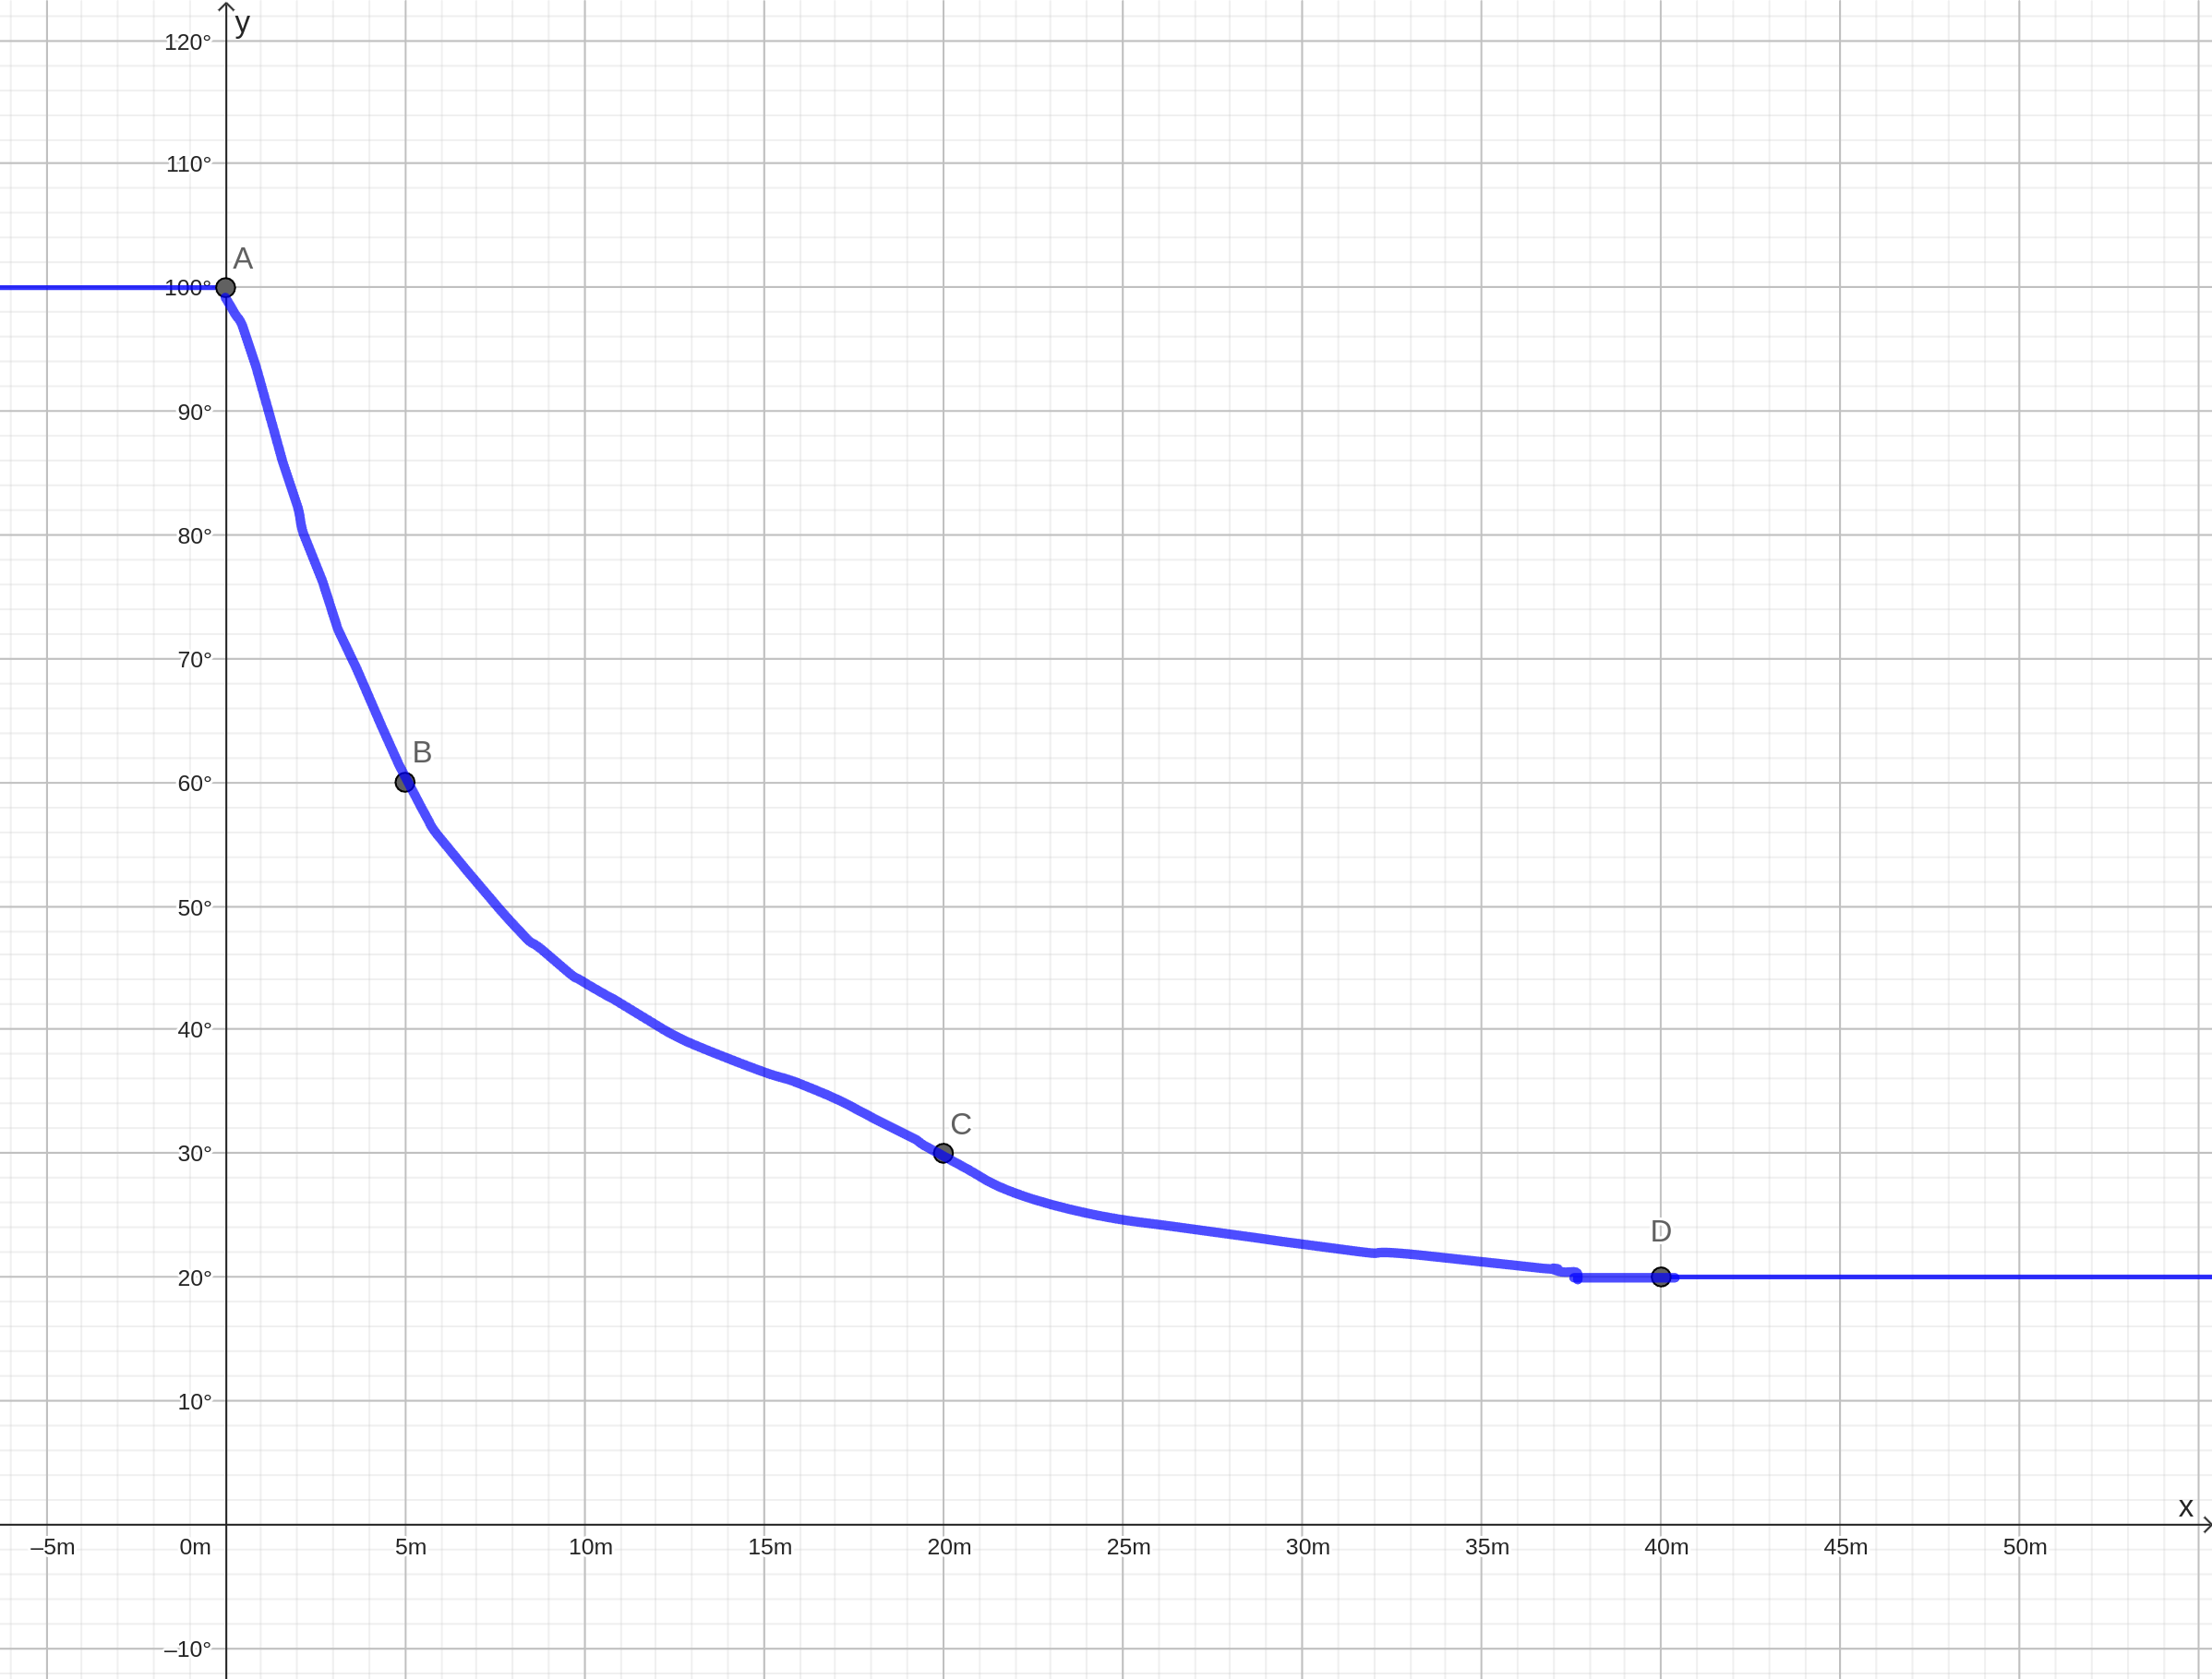
\includegraphics[scale=0.2]{../img/guide_01/ex_01.png} 
\centering
\label{fig:1}
\end{figure}

\end{document}
